\documentclass{beamer}
\usepackage[latin1]{inputenc}
\usetheme{Goettingen}
\title[SDF Crash Course]{Fault tolerance in Synchronous Dataflow}
\author{Nic Hollingum}
\institute{USYD}
\date{23 May, 2011}
\begin{document}

\begin{frame}
\titlepage
\end{frame}

%-----------------------------------------------------------------------------------
\section{Motivation}

\begin{frame}{Parallelism}
\begin{columns}
\begin{column}{6cm}
\begin{itemize}
	\item Chips cant handle speedup
	\item Move to parallelism, multicore, distributed, cloud
	\item SDF, paradigm allows explicit parallelism
	\item Map Reduce \cite{dea08}, StreaMIT \cite{thies02}
\end{itemize}
\end{column}
\begin{column}{4cm}
\center{
\includegraphics[height=7cm]{../res/Mapreduce.jpg}}
\caption{Marius Watz}
\end{column}
\end{columns}
\end{frame}

\begin{frame}{Fault Tolerance}
\begin{columns}
\begin{column}{4cm}
\center{
\includegraphics[height=7cm]{../res/computerfire.jpg}}
\end{column}
\begin{column}{6cm}
\begin{itemize}
	\item Computer death shouldnt require total recomputation
	\item Short mean time to failure (100 hours) \cite{ree06}
	\item Systems must prevent this failure:
	\begin{itemize}
		\item Work reassignment \cite{dea08}
		\item Checkpointing (databases)
		\item Task duplication
	\end{itemize}
\end{itemize}
\end{column}
\end{columns}
\end{frame}

%-----------------------------------------------------------------------------------
\section{Research Questions}

\begin{frame}{So...}
\begin{itemize}
	\item How can we best provide fault tolerance (FT)?
	\item How does the provision of FT affect runtim and bandwidth?
	\item Can tradeoffs be made using different FT Mechanisms?
	\item What are the properties of SDF that make this easier/harder?
	\item What assurances can be made to the users?
\end{itemize}
\end{frame}

%-----------------------------------------------------------------------------------
\section{Prior Work}

\begin{frame}{Scheduling}
\begin{columns}
\begin{column}{6cm}
\begin{itemize}
	\item Makespan optimization from Lenstra, Shmoys and Tardos \cite{len87}
	\item Communication cost reduction from Boykov, Veksler and Zabih \cite{boy01}
	\item Costs formulation from Stone \cite{sto77}
\end{itemize}
\end{column}
\begin{column}{4cm}
\center{
\includegraphics[height=7cm]{../res/schedule.jpg}}
\end{column}
\end{columns}
\end{frame}

\begin{frame}{Fault Tolerance}
\begin{itemize}
	\item Task reassignment from Mapreduce \cite{dea08}
	\item Software redundancies from Randell \cite{ran75}
	\item Task replication from Litke et al. \cite{lit07}
	\item Checkpoint recovery \cite{ree06}
\end{itemize}
\end{frame}

%-----------------------------------------------------------------------------------
\section{Methodology}

\begin{frame}{Methodology}
\begin{itemize}
	\item Formulate the assignment problem to include FT
	\item Generate approximations for the (NP-Hard) formulation
	\item Analyse the approximations, and the effect of FT on optimality
	\item Compare various FT mechanisms
	\item Use a simulator to analyse actual runnings
	\item For small enough graphs, compute IP to optimality and compare
\end{itemize}
\end{frame}

%-----------------------------------------------------------------------------------
\section{Plan}

\begin{frame}{Plan}
\center{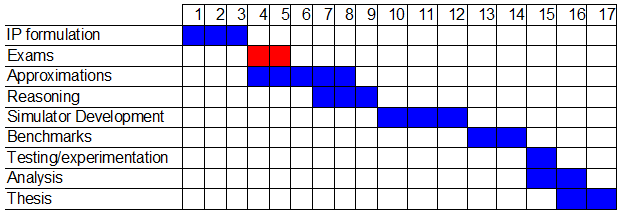
\includegraphics[height=7cm]{../res/gantt.png}}
\end{frame}

%-----------------------------------------------------------------------------------
\section{References}

\begin{frame}[allowframebreaks]{References}
\bibliographystyle{wmaainf}
\bibliography{biblio}
\end{frame}

\end{document}
